\subsection{Put All the Pieces Together --- Demonstration Plan}

We plan to build three systems to demonstrate our research
results: A content-based video scene retrieval system, a digital VCR
that supports both viewing and content interactivity, and
a multi-camera video surveillance system. 
The content-based scene retrieval system
provides the digital-VCR project with an
efficient storage and an effective query engine that can help
the viewer select content
before the viewer issues a fast-forward or replay command.
The digital VCR, which receives only
one stream at a time, in turn, is extended
by the multi-camera video surveillance project, which 
handles multiple cameras, streams and viewers simultaneously.

\subsubsection{A Content-based Video Scene Retrieval System}

The content-based search engine receives a query 
from a user. The query can consist of an image/drawing and 
some key words. The search engine profiles
the image/drawing, together with the specified
key words, and it finds the matching scenes in its repository
and returns them to the viewer in a ranking order.   
The key technologies demonstrated via this prototype are
1) the search engine's feature clustering and
indexing can scale well with respect to
the receiver's available resources and the size of
the database, and 2) the search engine can index 
features with different importance and can
cope with missing features.
%We will show that queries such as
%``Find all scenes in which a man is walking by a car''
%can be retrieved effectively.

{\bf Core technologies demonstrated}: 
feature clustering, indexing and query processing.

\subsubsection{A Digital VCR}

\begin{figure}[t]
\centerline{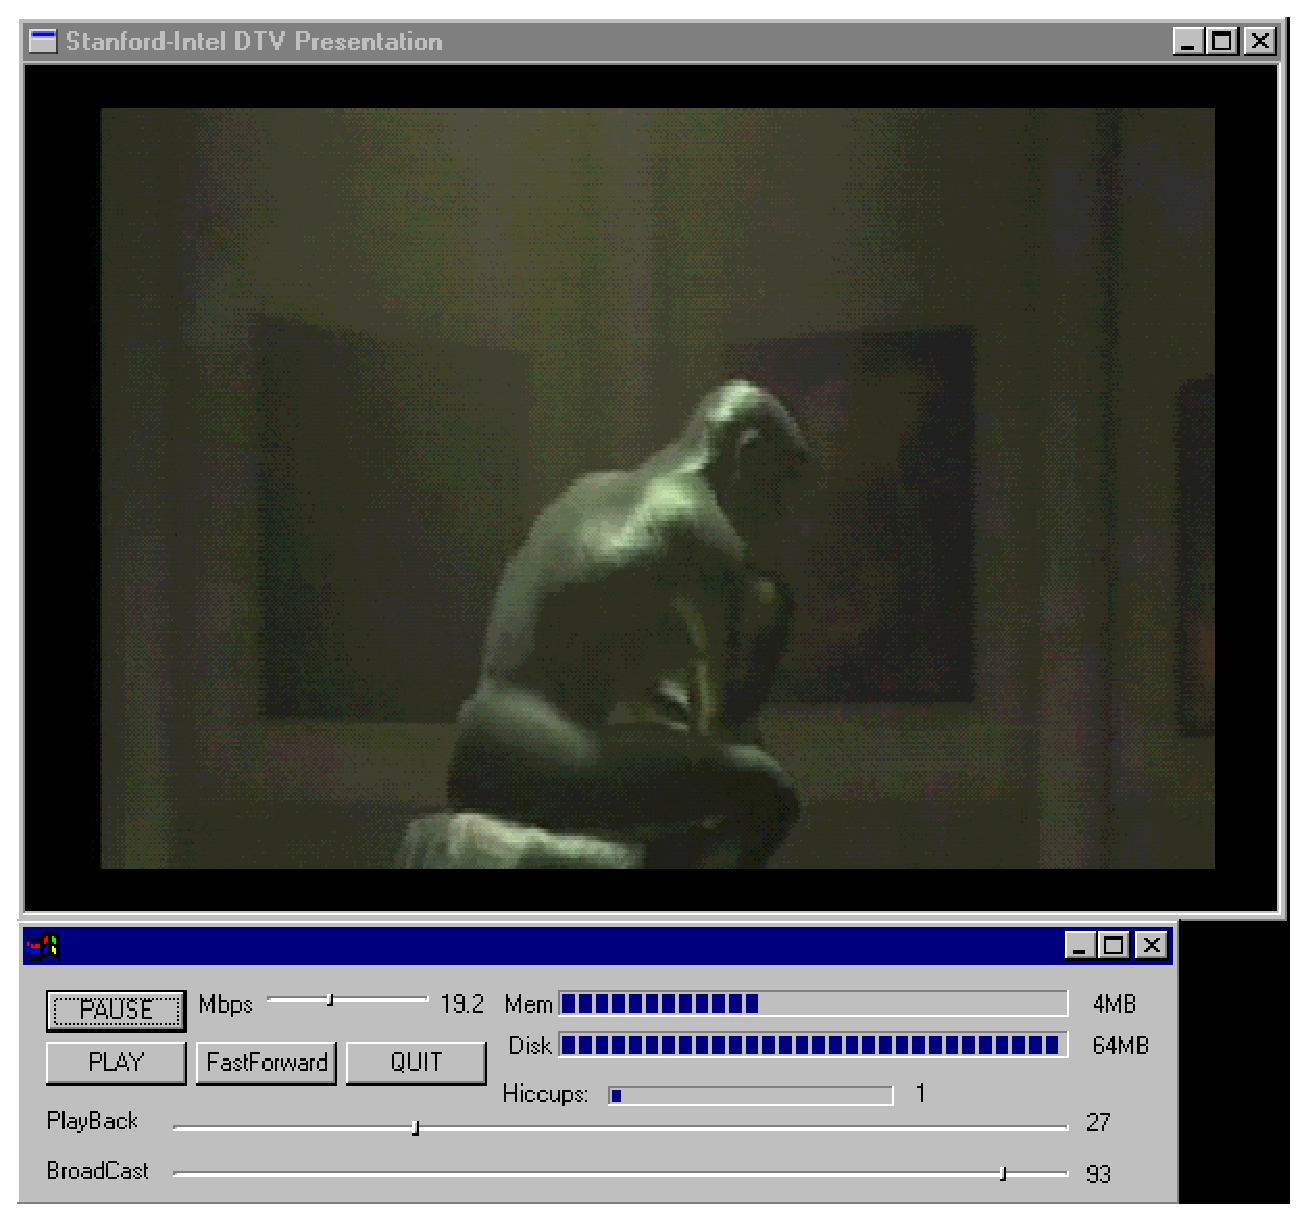
\psfig{figure=digital_vcr.ps,width=300pt,height=200pt}}
\caption{A Digital VCR Screen Shot.}
\label{fig-codec}
\end{figure}

The implementation of a
Digital VCR that supports VCR-like interactive functions including
{\em pause}, {\em fast-forward} and {\em instant replay} is under way.
Figure~\ref{fig-codec} shows a screen shot of the user interface
(i.e., {\em codec}) and display.
At the bottom of the figure is the codec through which a viewer
issues interactive commands and monitors the system.
To issue a command, a viewer selects and presses one
of the control buttons on the upper-left corner of
the codec (described shortly). To help visualize
the system, the codec uses trackbars to display various statuses. The five
trackbars from the top to the bottom on the codec keep track
of the amount of memory use, the amount of disk use,
the accumulated number of hiccups, the playback progress,
and the broadcast progress. 
In the final phase of this project we
will incorporate the content-based video scene search engine
into the digital VCR for supporting scene
queries before the viewer issues a fast-forward or replay request. 
                          
%When a viewer watches a TV program live, memory is
%used to buffer the mismatch between the data transmission
%rate and the playback rate. The memory trackbar keeps
%track of the current memory use. The disk use
%is zero when a program is watched live. When the pause button
%is pressed, the excessive data that the DRAM cannot stage is
%written onto the disk. Using the disk as a part of the
%cache, the VCR can allow the viewer to pause for a substantial amount
%of time (a $9.1$ GBytes disk can buffer more than one hour of
%$19.2$ Mbps DTV program).  After returning from the break, the viewer
%can press the {\em play} button to resume the playback. At
%this time, the decoder consumes data from the disk while the
%broadcast data continue arriving and being appended to
%the tail of the disk file. The viewer has the option to
%perform {\em fast-forward} to catch up with the live
%program. When the fast-forward button is pressed, the Digital VCR
%retrieves data from the disk at a faster pace and the decoder
%decodes and displays key frames only. The data cached on the disk are
%eventually used up and the playback returns to the
%live mode.  

{\bf Core technologies demonstrated}: 
caching, prefetching, data 
organization, and QoS-adaptive buffer management.

\subsubsection{A Multi-camera Video Surveillance System}

The most challenging application I propose here is a video
surveillance system.
In this application, video streams are captured 
using multiple video cameras.
For each stream, the 
foreground object is segmented from its background using range, color, 
motion, or other techniques. Then, the set of streams 
are compressed and transmitted to the receiver. 

In the receiver, on a screen, 
viewpoint control could be performed with a joy stick.
The challenge is being able to switch from one
camera to another with minimum
delay and being able to perform a time-shift
operation on one camera without affecting the
reception and recording of the other
cameras. The scene descriptions are created when 
streams arrive at the receiver. These descriptions
are time-stamped, indexed and stored in the database.
We will show that queries such as 
``Find all cars parked around
the facility on 1/1/99'' can be retrieved effectively.

{\bf Core technologies demonstrated}: 
buffer management handling
multiple simultaneous streams.

